\documentclass[11pt]{article}
\usepackage{geometry}
\geometry{letterpaper}

\usepackage{graphicx}
\usepackage{amssymb}
\usepackage{epstopdf}
\usepackage{natbib}
\usepackage{amssymb, amsmath}
\usepackage{listings}
\usepackage[final]{pdfpages}
\usepackage[framed,numbered,autolinebreaks,useliterate]{mcode}
\usepackage{tikz}
\usepackage{subfig}
\usepackage[underline=true,rounded corners=false]{pgf-umlsd}
\usepackage{tikz-uml}
\usetikzlibrary{mindmap}

\lstset{language=matlab}
\lstset{breaklines}
\lstset{extendedchars=false}
\DeclareGraphicsRule{.tif}{png}{.png}{`convert #1 `dirname #1`/`basename #1 .tif`.png}

%\title{Title}
%\author{Name 1, Name 2}
%\date{date}

\begin{document}



\thispagestyle{empty}

\begin{center}

\includegraphics[width=5cm]{ETHlogo.eps}

\bigskip


\bigskip


\bigskip


\LARGE{ 	Lecture with Computer Exercises:\\ }
\LARGE{ Modelling and Simulating Social Systems with MATLAB\\}

\bigskip

\bigskip

\small{Project Report}\\

\bigskip

\bigskip

\bigskip

\bigskip


\begin{tabular}{|c|}
\hline
\\
\textbf{\LARGE{A Generalized Model for Peer Review:}}\\
\textbf{\LARGE{Design and Implementation}}\\
\\
\hline
\end{tabular}
\bigskip

\bigskip

\bigskip

\LARGE{Xiang Gao}



\bigskip

\bigskip

\bigskip

\bigskip

\bigskip

\bigskip

\bigskip

\bigskip

Zurich\\
Dec 2011\\

\end{center}



\newpage

%%%%%%%%%%%%%%%%%%%%%%%%%%%%%%%%%%%%%%%%%%%%%%%%%

\newpage
\section*{Agreement for free-download}
\bigskip


\bigskip


\large We hereby agree to make our source code for this project freely available for download from the web pages of the SOMS chair. Furthermore, we assure that all source code is written by ourselves and is not violating any copyright restrictions.

\begin{center}

\bigskip


\bigskip


\begin{tabular}{@{}p{3.3cm}@{}p{6cm}@{}@{}p{6cm}@{}}
\begin{minipage}{3cm}

\end{minipage}
&
\begin{minipage}{6cm}
\vspace{2mm} \large Xiang Gao

\vspace{\baselineskip}

\end{minipage}
&
\begin{minipage}{6cm}

\end{minipage}
\end{tabular}


\end{center}
\newpage

%%%%%%%%%%%%%%%%%%%%%%%%%%%%%%%%%%%%%%%

% IMPORTANT
% you MUST include the ETH declaration of originality here; it is available for download on the course website or at http://www.ethz.ch/faculty/exams/plagiarism/index_EN; it can be printed as pdf and should be filled out in handwriting
% 
\includepdf[pages={1}]{declare.pdf}

%%%%%%%%%% Table of content %%%%%%%%%%%%%%%%%

\tableofcontents

\newpage

%%%%%%%%%%%%%%%%%%%%%%%%%%%%%%%%%%%%%%%

\section{Introduction and Motivations}
In this paper, we will investigate the modeling of peer review process. There are not many existing papers on the modeling of peer review. In 2010, Thurner \cite{thurner2010peer} implemented a simple model and argued that a small fraction of rational referee will decrease the quality of publication obviously. Francisco \cite{grimaldoproposal} implemented a model called PR-1 which is a subset of their proposed model PR-M and their experiments showed that three reviewers are enough to perform a good selection. 

The author of this paper intended to extend the existing model to a new one, but due to the time limitation and the author's ability, we only implemented a small prototype. The contribution of this paper is two fold, one is to define the six building blocks for modeling peer review, these core concepts could be the foundation for further research. Another contribution is to develop a small code framework based on the six building blocks, which could be reused, extended by other researchers so as to speed up the development of programs. We do not give any detail model or implementation about peer review process, so we call this model a generalized model. This decision is to give other people who want to extend existing model or idea more flexibility.

The rest of paper is organized as follows, we first define the six building blocks for peer review, next we describe in detail about the implementation, then we show an example model based on the building blocks and code framework, at last we conclude the paper.

\newpage

\section{Six Building Blocks for Modeling Peer Review}

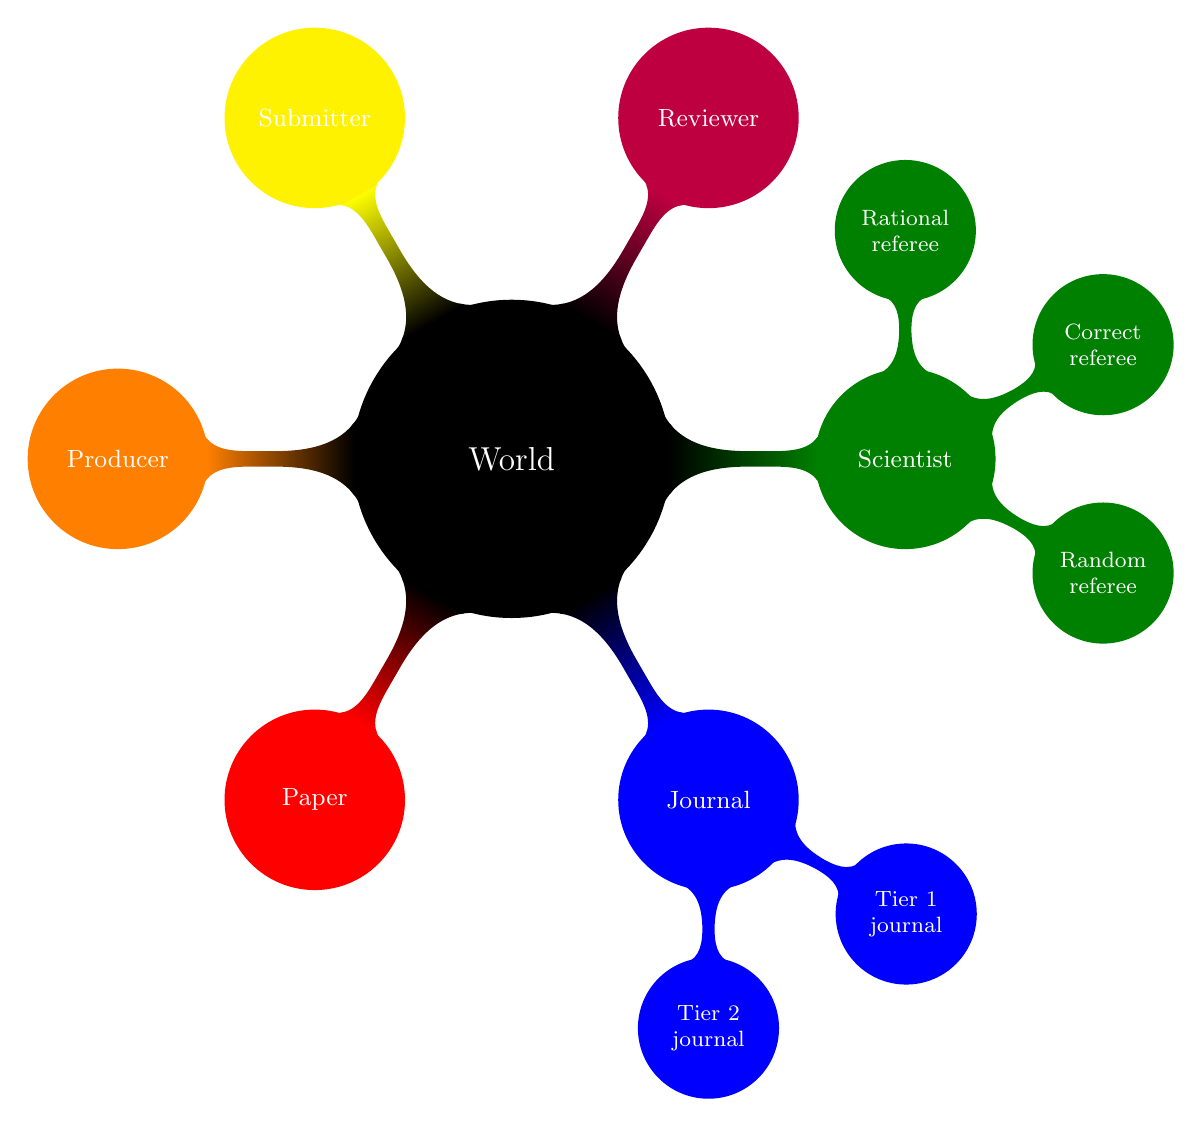
\begin{tikzpicture}[]
  \path[mindmap,concept color=black,text=white]
    node[concept] {World}
    [clockwise from=0]
    child[concept color=green!50!black] {
      node[concept] {Scientist}
      [clockwise from=90]
        child { node[concept] {Rational referee} }
        child { node[concept] {Correct referee} }
        child { node[concept] {Random referee} }
    }
    child[concept color=blue] {
    node[concept] {Journal}
    [clockwise from=-30]
      child { node[concept] {Tier 1 journal} }
      child { node[concept] {Tier 2 journal} }
    }
    child[concept color=red] { node[concept] {Paper} }
    child[concept color=orange] { node[concept] {Producer} }
    child[concept color=yellow] { node[concept] {Submitter} }
    child[concept color=purple] { node[concept] {Reviewer} };
\end{tikzpicture}

In the academic world, scientists, papers, and journals are three important entities. Scientists produce papers, submit papers to journals for review, after receiving the manuscript, the journal will arrange other scientists to review papers and decide if the papers are accepted, rejected, or revision. These three entities constitutes three building blocks in the peer review process.

The other three building blocks are not concrete entities, but three algorithms or methods. One is called producer, which defines the quality of the paper produced by a scientist, another one is called submitter, which decides which journal the scientist wants to submit his or her paper. The last one is named reviewer, this is the method journals use to review and accept papers.

These concepts are not new, but are extracted from existing models. Most of the existing research try to use agent based model to simulate the peer review process, when come to the implementation, they must decide the three algorithms we defined as building blocks. Different models employ different algorithms for the three algorithm building blocks and use different attributes of the three entity building blocks. Each one of the building blocks can be designed separately, and you can run a lot of experiments with differently combinations. This will result in a lot of work to find the best method to implement the peer review (many researcher aim to find a good way to improve the peer review), which is far beyond the capability of the author. Therefore we focus to implement a small prototype to illustrate the framework we propose and show an example to the user how to extend the model. Hopefully, this work will help others save some efforts when design the model and implement it.

\newpage

\section{Implementation}

\subsection{Class design}

\begin{figure}[h]
\begin{tikzpicture}
\begin{umlpackage}{Common}
\umlclass{Scientist}{
  id  \\ intelligence
}{
  produce\_paper(Producer) : Paper\\
  submit\_paper(Submitter)
}

\umlclass[y=-3]{Paper}{
  id \\ quality
}{}

\umlclass[y=-7]{Journal}{
  id \\ impact
}{
  review\_paper(Reviewer)
}

\umlclass[x=5,y=-3]{World}{
  Scientist \\ Journal
}{
  simulate\_world(Simulator)
}

\umlinterface[x=5,y=-7]{Simulator}{}{
  simulate(World)
}

\umlinterface[x=10,y=0]{Producer}{}{
  produce(Scientist)
}

\umlinterface[x=10,y=-3]{Submitter}{}{
  submit(Paper)
}

\umlinterface[x=10,y=-7]{Reviewer}{}{
  review(Journal, Paper)
}

\end{umlpackage}
\end{tikzpicture}
\end{figure}

This part details the implementation of our generalized model. The six building blocks are defined as classes in MATLAB. Scientists have attributes such as id and intelligence, they can produce paper, and submit paper. Paper has name, quality attributes, and other attributes if you think useful, i.e. a unique id to identify the paper for the journal, the citation number, references, co-authors. Journal has attributes like impact factors, editors, committees and so on.

Producer defines an interface called produce, submitter has an interface called submit, reviewer has an interface called review. The three algorithm are defined as abstract classes in MATLAB. Any specific model must implement their own algorithm for these three building blocks.

World is a mashup of all the components in the academic world, which is defined as a class. Simulator provides the the simulation algorithm to simulate the peer review process. All these are shown in the class diagram.

\subsection{Work Flow}

\begin{figure}[h]
  \centering
  \begin{sequencediagram}
    \newthread{sci}{Scientist}
    \newinst{pro}{Producer}
    \newinst{pp}{Paper}
    \newinst{sub}{Submitter}
    \newinst{jor}{Journal}
    \newinst{rev}{Reviewer}

    \begin{sdloop}{Run Loop}
      \begin{call}{sci}{produce\_paper()}{pro}{paper}
        \begin{callself}{pro}{produce()}{}
        \end{callself}
      \end{call}
      \begin{call}{sci}{submit\_paper()}{sub}{journal}
        \begin{callself}{sub}{submit()}{}
        \end{callself}
      \end{call}
      \begin{call}{jor}{review\_paper()}{rev}{decision}
        \begin{callself}{rev}{review()}{}
        \end{callself}
      \end{call}
    \end{sdloop}
  \end{sequencediagram}

  \caption{Work flow of simulation.}
\end{figure}

This section we briefly describe the flow of our simulation process. Although we do not intend to give any specific algorithm for the simulate process, since the framework is mainly designed for agent based model, we put it here for the sake of completeness. In every iteration, scientists first produce papers, and then submit papers to the journals. Journal will arrange reviewers to review the paper and make the final decision. The detail process should be self-evident from the sequence diagram above.

\newpage

\section{Example}
Now we show an example based on the framework, specifically, we implement Thurner's model \cite{thurner2010peer}. The detail model can be found in Thurner's paper. In the following we reproduce all the results appeared in his paper.

\begin{figure}[!th]
    \centering
    \subfloat[][]{\resizebox{7cm}{!}{\includegraphics{../figure/Thurner/avg_quality_100_0_0.eps}}}
    \qquad
    \subfloat[][]{\resizebox{7cm}{!}{\includegraphics{../figure/Thurner/accept_quality_100_0_0.eps}}}
    \caption{(a) the average paper quality when all the reviewers are correct ones. (b) the distribution of quality for submitted paper and accepted paper}
    \label{fig:cont}
\end{figure}

\begin{figure}[!th]
    \centering
    \subfloat[][]{\resizebox{7cm}{!}{\includegraphics{../figure/Thurner/avg_quality_90_0_10.eps}}}
    \qquad
    \subfloat[][]{\resizebox{7cm}{!}{\includegraphics{../figure/Thurner/accept_quality_90_0_10.eps}}}
    \caption{(a) the average paper quality when 90 percent the reviewers are correct ones and 10 percent are rational. (b) the distribution of quality for submitted paper and accepted paper}
    \label{fig:cont}
\end{figure}

\begin{figure}[!th]
\begin{center}
\resizebox{10cm}{!}{\includegraphics{../figure/Thurner/no_network_comparison.eps}}
\caption{comparison of average paper quality when varying the fraction of random reviewers from 0 to 0.2, the fractional of rational reviewers from 0 to 0.7}
\end{center}
\end{figure}

\begin{figure}[!th]
\begin{center}
\resizebox{10cm}{!}{\includegraphics{../figure/Thurner/network_comparison.eps}}
\caption{comparison of average paper quality of when 10 percent scientists are in network and varying the fractional of rational reviewers from 0 to 0.7}
\end{center}
\end{figure}

\begin{figure}[!th]
\begin{center}
\resizebox{10cm}{!}{\includegraphics{../figure/Thurner/journal_comparison.eps}}
\caption{Effect of journal favors higher quality papers.}
\end{center}
\end{figure}

\newpage

\section{Lessons and Experiences}

\newpage

\bibliography{report}
\bibliographystyle{plain}

\newpage

\appendix
\section{Source Code}

\lstinputlisting{../../code/OO/common/World.m}
\lstinputlisting{../../code/OO/common/Simulator.m}
\lstinputlisting{../../code/OO/common/Scientist.m}
\lstinputlisting{../../code/OO/common/Journal.m}
\lstinputlisting{../../code/OO/common/Paper.m}
\lstinputlisting{../../code/OO/common/Producer.m}
\lstinputlisting{../../code/OO/common/Submitter.m}
\lstinputlisting{../../code/OO/common/Reviewer.m}

\lstinputlisting{../../code/OO/example/ThurnerModel.m}
\lstinputlisting{../../code/OO/example/ThurnerWorld.m}
\lstinputlisting{../../code/OO/example/ThurnerSimulator.m}
\lstinputlisting{../../code/OO/example/ThurnerScientist.m}
\lstinputlisting{../../code/OO/example/GaussianProducer.m}
\lstinputlisting{../../code/OO/example/NaiveSubmitter.m}
\lstinputlisting{../../code/OO/example/RandomReviewer.m}
\end{document}
